\section{Corrected search: complete outcomes and retained incumbents}
\label{sec:native-corrected-choice-results}

\subsection{All four-step paths, including the execution null}
The original writer closes on November 17, 2026, at 02:20:21 UTC; its
supervisor records exit zero at 02:20:24 UTC. All 24 own attempts and three
fresh references are present. Twenty-three own outcomes complete and one
remains an original execution null. Eight complete own outcomes tie their
assigned visible reference, 15 worsen it and none improves it. No attempt is
repaired, replaced, omitted or given an imputed failure loss.

Table~\ref{tab:corrected-choice-full-paths} contains every own assigned loss,
not only selected candidates. Its six rows are coupled search histories on
one reused world condition, not six independent scientific populations.
Within each objective, uniform and adaptive generation-zero programs are
literal matches but separately executed worlds. Three later adaptive moves
are actual feedback-conditioned proposals; the four uniform proposals are
initial random samples with loss-based selection. The comparisons remain
end-to-end search packages, not isolated representation or equal-compute effects.

\begin{table}[t]
\centering\small
\setlength{\tabcolsep}{5pt}
\begin{tabular}{llrrrrrr}
\toprule
Method & Target & Reference & $g=0$ & $g=1$ & $g=2$ & $g=3$ & Best own\\
\midrule
Uniform & U & $-28.67$ & $-27.67$ & $-28.33$ & $-27.67$ & $-28.33$ & $-28.33$\\
Adaptive & U & $-28.67$ & $-27.67$ & $-25.67$ & $-28.33$ & $-26.67$ & $-28.33$\\
Free & U & $-28.67$ & $-7.00$ & null & $-28.67$ & $-28.67$ & $-28.67$\\
Uniform & C & $-12.67$ & $-9.67$ & $-10.33$ & $-10.67$ & $-12.33$ & $-12.33$\\
Adaptive & C & $-12.67$ & $-9.67$ & $-12.67$ & $-11.67$ & $-12.67$ & $-12.67$\\
Free & C & $-12.67$ & $-12.67$ & $-12.67$ & $-12.67$ & $-12.67$ & $-12.67$\\
\bottomrule
\end{tabular}
\caption{All 24 own attempts in the corrected native study. Lower assigned loss
is better. Exact retained floats, not displayed rounding, govern selection.
The null has unavailable loss, not zero or an infinite penalty. Best own excludes
the measured warm reference; best known includes it and never leaves the
reference level in this study. This is not an independent method-ranking sample.}
\label{tab:corrected-choice-full-paths}
\end{table}

\begin{figure}[t]
\centering
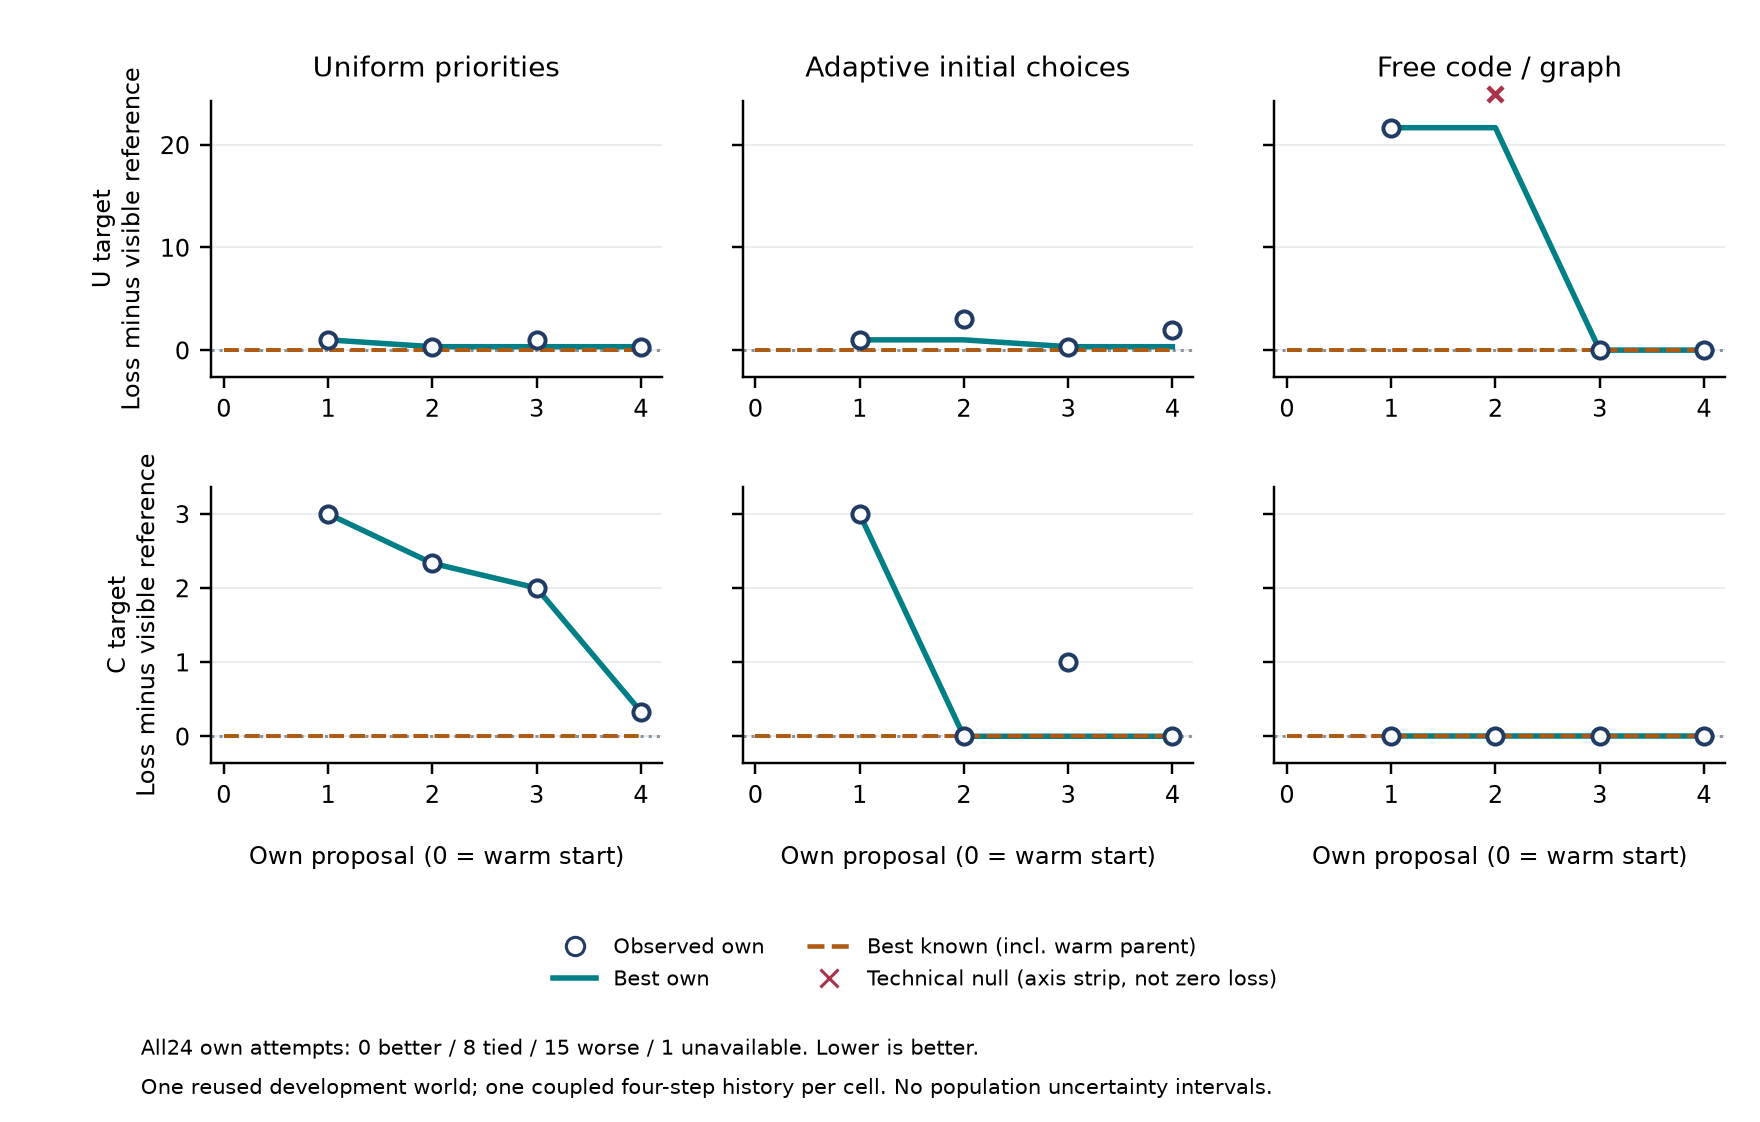
\includegraphics[width=\linewidth]{../research/figures/native-corrected-choice-search-v1/corrected-choice-loss-paths.png}
\caption{Complete corrected search paths, relative to each assigned measured
reference. Open circles show actual own losses, teal lines the best complete
own proposal and dashed orange lines best known including the warm reference.
The execution null is marked above its panel, not plotted as zero loss. Both
rendering runs produce identical PNG/SVG bytes from the original closed readout.
One coupled development condition is shown; no confidence interval or independent
method superiority is inferred.}
\label{fig:corrected-choice-loss-paths}
\end{figure}

Several paths recover their own earlier loss without improving best known.
Adaptive C moves from $-9.6667$ to $-12.6667$ at its first update, matching
the supplied terminal reference. Its next update worsens, and its last ties
again. Uniform C reaches its best own loss at its fourth sample, still about
$1/3$ worse than the reference. Free U recovers from $-7$ and an execution
null to the known $-28.6667$ reference level. These are observed search paths,
not new best-known discoveries or demonstrated causal benefits of feedback.
The adverse and repeated proposals remain informative records rather than
reasons to refill the declared budget.

\subsection{The returned policy is not necessarily an invented policy}
The original writer freezes both endpoint scopes before any unused-condition
evaluation. Every primary best-known endpoint returns a measured visible
reference: the priority-zero policy for U and terminal-priority-zero policy
for C. The six logical labels therefore return two supplied policies, not six
independently invented institutions. They are genuine measured incumbents,
not fabricated fallback losses, and the separate own-only results remain visible.

\begin{table}[t]
\centering\small
\setlength{\tabcolsep}{5pt}
\begin{tabular}{llrlr}
\toprule
Method & Target & First best own $g$ & Primary origin & Own minus reference\\
\midrule
Uniform & U & 1 & supplied priority-zero & $+1/3$\\
Adaptive & U & 2 & supplied priority-zero & $+1/3$\\
Free & U & 2 & supplied priority-zero & $0$\\
Uniform & C & 3 & supplied terminal-zero & $+1/3$\\
Adaptive & C & 1 & supplied terminal-zero & $0$\\
Free & C & 0 & supplied terminal-zero & $0$\\
\bottomrule
\end{tabular}
\caption{Literal earliest-minimum selection from the original completed study.
All six primary endpoints tie their measured reference by retaining it.
Among six separate own-only endpoints, three tie and three worsen the reference.
An exploratory sample does not make the best-known incumbent worse, but
retaining a supplied incumbent is not useful autonomous invention.}
\label{tab:corrected-choice-frozen-endpoints}
\end{table}

The exact frozen selection is retained independently of manuscript prose:
its content checksum is
\code{358c6a22e75b540c}\allowbreak\code{c8170f3d4e283876}\allowbreak
\code{40d57bb13ac16bec}\allowbreak\code{e2b3cdc48b7ab609}.
Changing the displayed table cannot change those programs, origins or tie rules.
Fixed-condition evaluation must reuse them literally. It would evaluate fixed
policies, not create independent optimizer replications or retroactively make
a reference an own submission.

\subsection{Source edits, invoked rules and researcher behavior are different layers}
All eight free-author sessions explicitly submit after 14 operations each.
A passive reader verifies their complete original binding, chronological
dispatch/completion chains and terminal file hashes twice, with byte-identical
outputs. The 112 original completed actions include 25 applied source edits.
Nineteen incremental changed-node rows have the same normalized Python AST
and six have a different AST; no connection or schedule edit occurs. These
are edit counts, not 25 candidate worlds, 19 distinct unchanged programs or
six useful invented algorithms. Other supported forms of design remain allowed.

That observation is more precise than claiming that all free edits are
formatting. For example, the final free U proposal replaces conditional native
acceptance with constant acceptance. Its source AST differs from the parent,
and four original annual selection receipts join bijectively to committed
native execution events. Its final portable checkpoint contains the submitted
candidate exactly. Nevertheless, the parent's actual current rule is already
accept-all, and all 179 recorded scientist request payloads and response-choice
sequences match the measured priority-zero reference. Provider response bodies
differ and their hashes are checked. This is an observed repeated trajectory,
not global program equivalence; source change and actual invocation are not
sufficient evidence of changed researcher behavior.

The first free U proposal is different in another way: its agenda source
actually favors longer catalog projects, despite its accompanying explanation.
Its 10 accepted decisions and $U=7$ are worse than the parent's 36 decisions
and $U=28.6667$. The next submitted U program has a double payload envelope:
local component returns do not establish downstream native paper-ID coverage,
and the original native outcome has unavailable loss. Neither the explanation
nor the probe result repairs that submitted program. In the later C sessions,
planned parameter/threshold changes are not implemented; literal source edits
preserve other configuration and, in the recorded cases, the parent's AST.

The passive edit analysis adds no production prompt, model call, code execution
or candidate gate. Equal AST never forbids a design, and different AST never
certifies usefulness. A genuine numerical topic-priority change remains visible
despite identical source AST. These observations motivate more consequential
proposal procedures; they do not themselves demonstrate that new diagnostic
feedback improves invention or identify intrinsic designer competence as the cause.

\subsection{Content support and physical cost}
The complete content export retains 910 accepted occurrences across 26 complete
physical worlds: 734 have positive centered panel utility, 176 have zero and
none has negative utility. There are 88 content hashes across worlds and no
within-world repeated content. Cross-world sharing is not within-world score
inflation or independent replication. Deleting fixed scored records alone
therefore cannot increase their summed U, holding all other consequences fixed;
this is not an attainable dynamic counterfactual or a global policy bound.

The terminal-priority-zero reference has $U=28.6667$ and collected $K=160$.
Every complete own outcome has no greater U and no lower K. This reference
weakly dominates all 23 complete own points on the observed U--K support.
Consequently, re-ranking this archive under $-U+\lambda K$ for any
$\lambda\geq0$ cannot place an own point strictly ahead of that reference.
The statement concerns these observed points only, not all executable policies.
It explains why merely changing the cost coefficient after this study is not
evidence of a newly discovered institutional tradeoff. Finding such a tradeoff
requires consequential new proposals or a separately justified objective, not
retuning a coefficient to claim a retrospective win.

\begin{table}[t]
\centering\small
\begin{tabular}{lrrr}
\toprule
Recorded physical component & Calls/replies & Prompt count & Output count\\
\midrule
Scientist complete replies & 4,650 & 7,016,180 & 425,437\\
Designer execution-readiness & 258 & 5,456,852 & 12,605\\
Designer authoring operations & 112 & 4,230,690 & 27,012\\
Common-content observer POSTs & 264 & --- & ---\\
Empty-prompt model loads & 44 & unknown & unknown\\
\bottomrule
\end{tabular}
\caption{Physical call components of the original development campaign,
not per-method equal-compute budgets. Scientist counts use provider-reported
tokens; designer counts use backend-native prompt/evaluation counts. Cached
prompt counts are subsets and are not added again. The observer's call count
does not assert comparable token accounting. Seventeen designer and 27 scientist
loads are separate from generation. Missing costs remain unknown.}
\label{tab:corrected-choice-physical-cost}
\end{table}

The scientist's reported token total is 7,441,617, including the reported
1,113,278 cached prompt tokens as a subset of prompt counts. No recorded
scientist wire input lacks its committed reply. The original supervisor spans
approximately 9 hours 19 minutes on a shared host. This is not a dedicated
hardware throughput benchmark; nested transport/provider durations must not be
summed into total wall time, GPU FLOPs, energy, money or an exclusive-resource
speed estimate. Generated proposals, readiness controls, probes and physical
world evaluation remain distinct costs.

\subsection{Closed development evidence, not yet unused-condition inference}
All seven original analysis chains now close normally: paired native cold
audits/costs, all-slot readouts, author outcomes, author visibility, native
source/consumer/resource effects, loss paths and signed-content exports.
Their paired files agree byte-for-byte. These are original-source analyses of
the unchanged scientific run, not newly generated candidates or observations.

The selection-fixed public/native software test also completes: actual native
execution with SCRIPTED HTTP, corpus and supervision processes 14 physical
evaluation worlds, 15 logical labels and 30 logical rows, with 120 paired
contrast rows. Its paired audits/costs/readouts match and the single full-path
test passes in approximately 23 minutes. It makes no real model calls and
does not consume scientific reserved conditions. The outer subprocess CLI
routing is outside this check. Software verification is not scientific gain.

The strict unused-condition inventory remains unresolved: exact metadata-bearing
SCRIPTED fixtures use one proposed seed, while old fixture stores and directory
symlinks produce coverage errors. No directory-name exemption, silent condition
switch or assertion of unusedness is applied. No real selection-fixed evaluation
is reported here and no original result is reselected using evaluation outcomes.
An important supported main-track claim and adequate independent evidence remain
research obligations, not consequences of another valid pilot.
